



\begin{figure*}[t]
	\centering
    \begin{subfigure}[t]{\columnwidth}
		\centering        
		%\includegraphics[trim={.5cm 13.7cm 13.5cm .5cm},clip,width=\textwidth]{figures/ann1}
		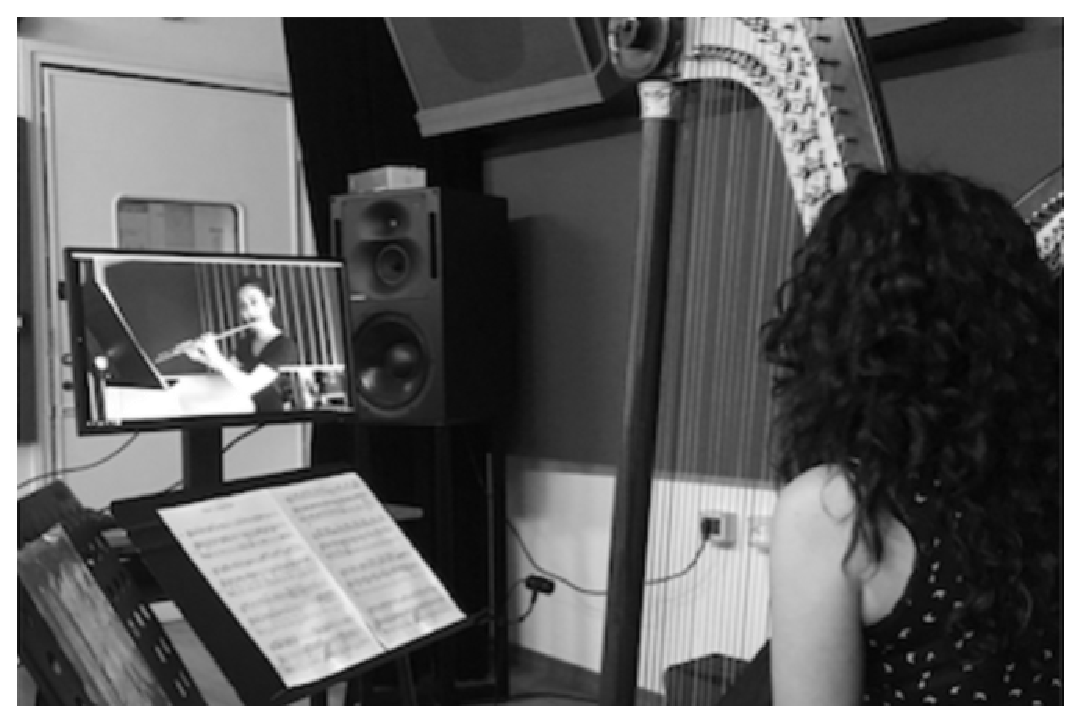
\includegraphics[width=\textwidth]{img/as.eps}
		\caption{View of Room 1}
		\label{subfig:as}
	\end{subfigure}
    \begin{subfigure}[t]{\columnwidth}
	\centering        
	%\includegraphics[trim={.5cm 13.7cm 13.5cm .5cm},clip,width=\textwidth]{figures/ann1}
	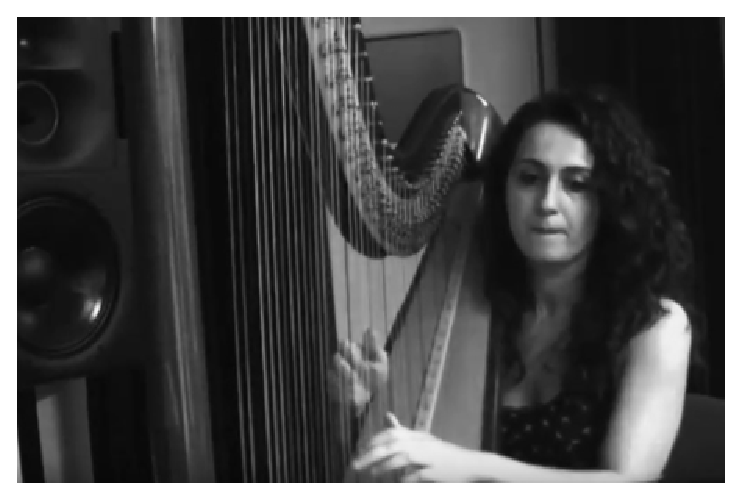
\includegraphics[width=\textwidth]{img/av.eps}
	\caption{View of Musician 1 from Room 2}
	\label{subfig:av}
	\end{subfigure}
    \begin{subfigure}[t]{\columnwidth}
	\centering        
	%\includegraphics[trim={.5cm 13.7cm 13.5cm .5cm},clip,width=\textwidth]{figures/ann1}
	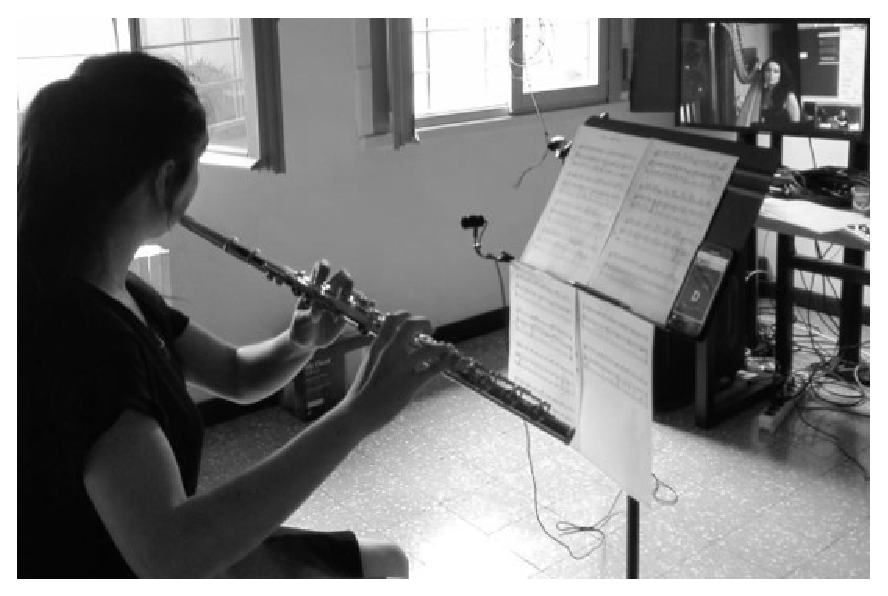
\includegraphics[width=\textwidth]{img/fs.eps}
		\caption{View of Room 2}
	\label{subfig:fs}
	\end{subfigure}
	\begin{subfigure}[t]{\columnwidth}
	\centering        
	%\includegraphics[trim={.5cm 13.7cm 13.5cm .5cm},clip,width=\textwidth]{figures/ann1}
	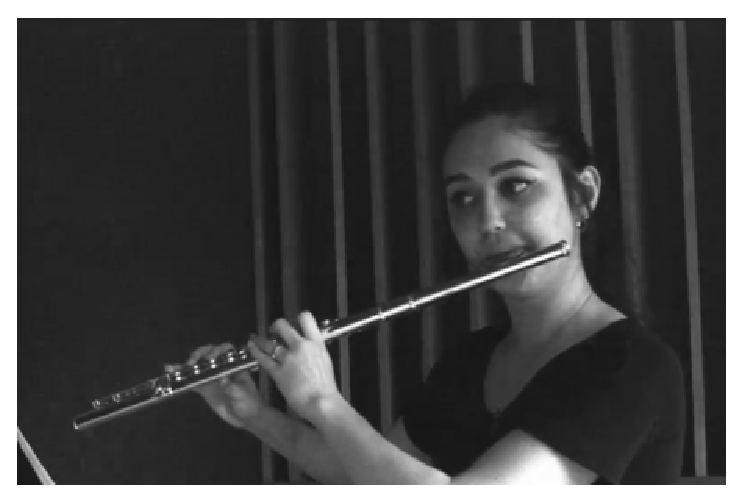
\includegraphics[width=\textwidth]{img/fv.eps}
	\caption{View of Musician 2 from Room 1}
	\label{subfig:fv}
\end{subfigure}

	\quad 
	\caption{View of Rooms 1 and 2 and the corresponding view seen on the screen}\label{fig:afsv}

\end{figure*}

